\documentclass[a4paper]{article}
\usepackage{amsmath,amssymb,caption,enumitem,float,geometry,graphicx,indentfirst,minted,parskip,tabularx,xcolor}
\usepackage[utf8]{inputenc}
\usepackage[english]{babel}
\usepackage[backend=bibtex]{biblatex}
\addbibresource{Lab3.bib}
\captionsetup[figure]{labelsep=period}
\captionsetup[listing]{labelsep=period}
\definecolor{bg}{rgb}{0.95,0.95,0.95}
\geometry{left=3.5cm,right=3.5cm,top=3.3cm,bottom=3.3cm}
\setlength{\parindent}{2em}
\usemintedstyle{emacs}
\begin{document}
\begin{titlepage}
    \vspace*{0.25cm}
    \noindent\rule[0.25\baselineskip]{\textwidth}{1pt}
    \begin{center}
        \huge{\textsc{UM--SJTU Joint Institute}}\vspace{0.3em}\\
        \huge{\textbf{System-on-Chip Design (ECE4810J)}}\vspace{0.3em}\\
        \noindent\rule[0.25\baselineskip]{\textwidth}{1pt}
    \end{center}
    \begin{center}
        \vspace{5cm}
        \Large{\textsc{Laboratory Report}}\vspace{0.5em}\\
        \Large{\textbf{Lab 3. PYNQ Overlays}}\vspace{1em}\\
        \Large{\textbf{Group 2}}\\
    \end{center}
    \vfill
    \large
    \begin{tabular}{ll}
        Name: Haochen Wu \hspace*{2em}&ID: 518021910558\hspace*{2em}\\
        Name: Siyuan Zhang \hspace*{2em}&ID: 518370910180 \hspace*{2em}\\
        Name: Yihua Liu \hspace*{2em}&ID: 518021910998\hspace*{2em}\\
        \\
        Date: \today
    \end{tabular}
\end{titlepage}
\tableofcontents
\newpage
\section{Overview}
In this lab, we will learn about PYNQ overlays. The goals of this lab are to:
\begin{itemize}
    \item Load overlay, use overlay and create overlay.
\end{itemize}
\section{Loading an overlay}
All the available overlays for the Arty Z7 boards:
\begin{itemize}
    \item Base Overlay
    \item Logictools Overlay
\end{itemize}
Under \texttt{/usr/local/lib/python3.6/dist-packages/pynq/overlays}, there are \texttt{base}, \texttt{\_\_init\_\_.py}, \texttt{logictools}, and \texttt{\_\_pycache\_\_}, so all the available overlays for the Arty Z7 boards are base overlay and logictools overlay \cite{pynqdoc251}.

Once we instantiate the base overlay, we use \texttt{help(base\_overlay)} command to know IPs and methods available, which is:
\begin{figure}[H]
    \centering
    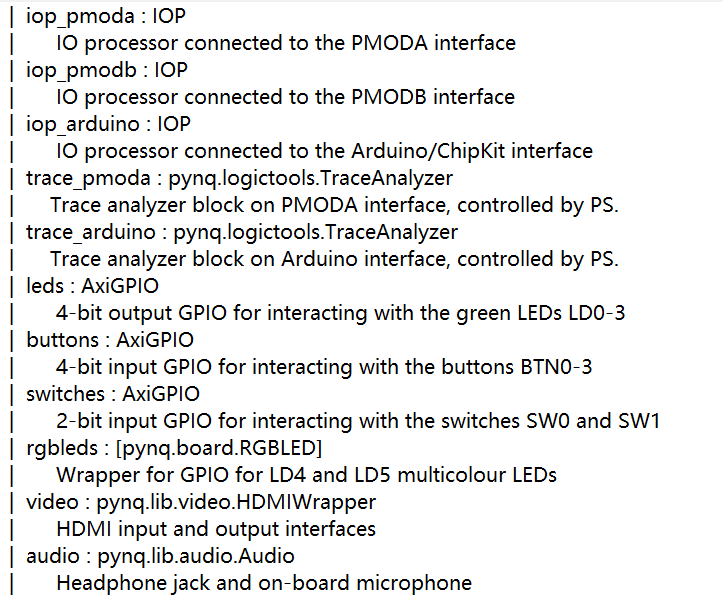
\includegraphics[width=1\textwidth]{1-2.png}
    \caption{Screenshot of available IPs in base overlay}
\end{figure}

\section{Partial Reconfiguration}
\subsection{Preparing the Files}
In this section, we use the demo files provided by the professor, as included in this example \cite{partialReconfig}.
\subsection{Loading Full Bitstream}
\begin{figure}[H]
    \centering
    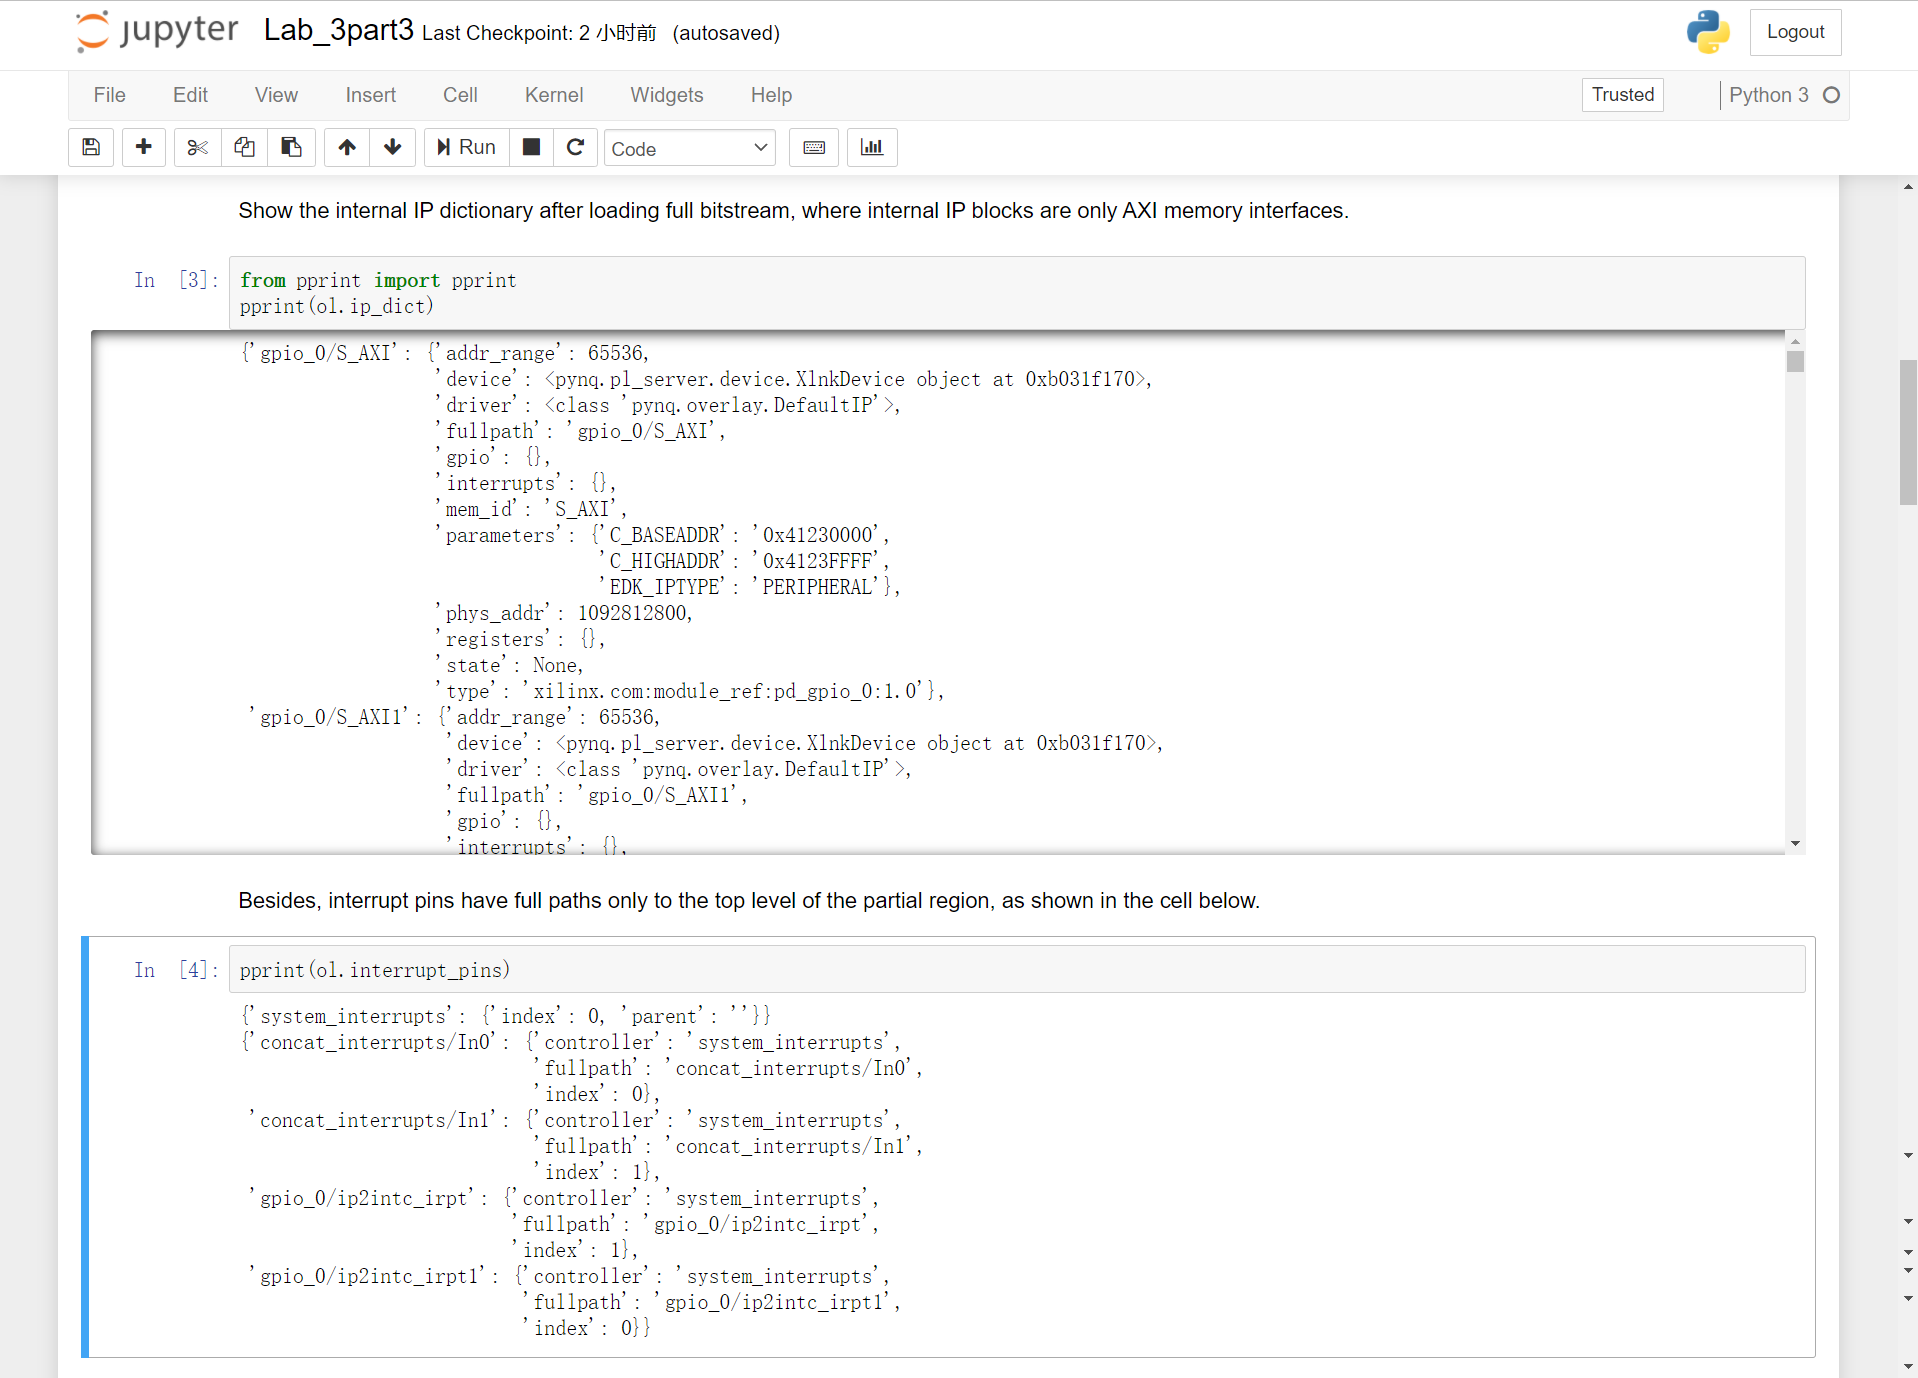
\includegraphics[width=1\textwidth]{1.png}
    \caption{Screenshot that shows full bit stream is loaded.}
\end{figure}
\subsection{Loading Partial Bitstream}
\begin{figure}[H]
    \centering
    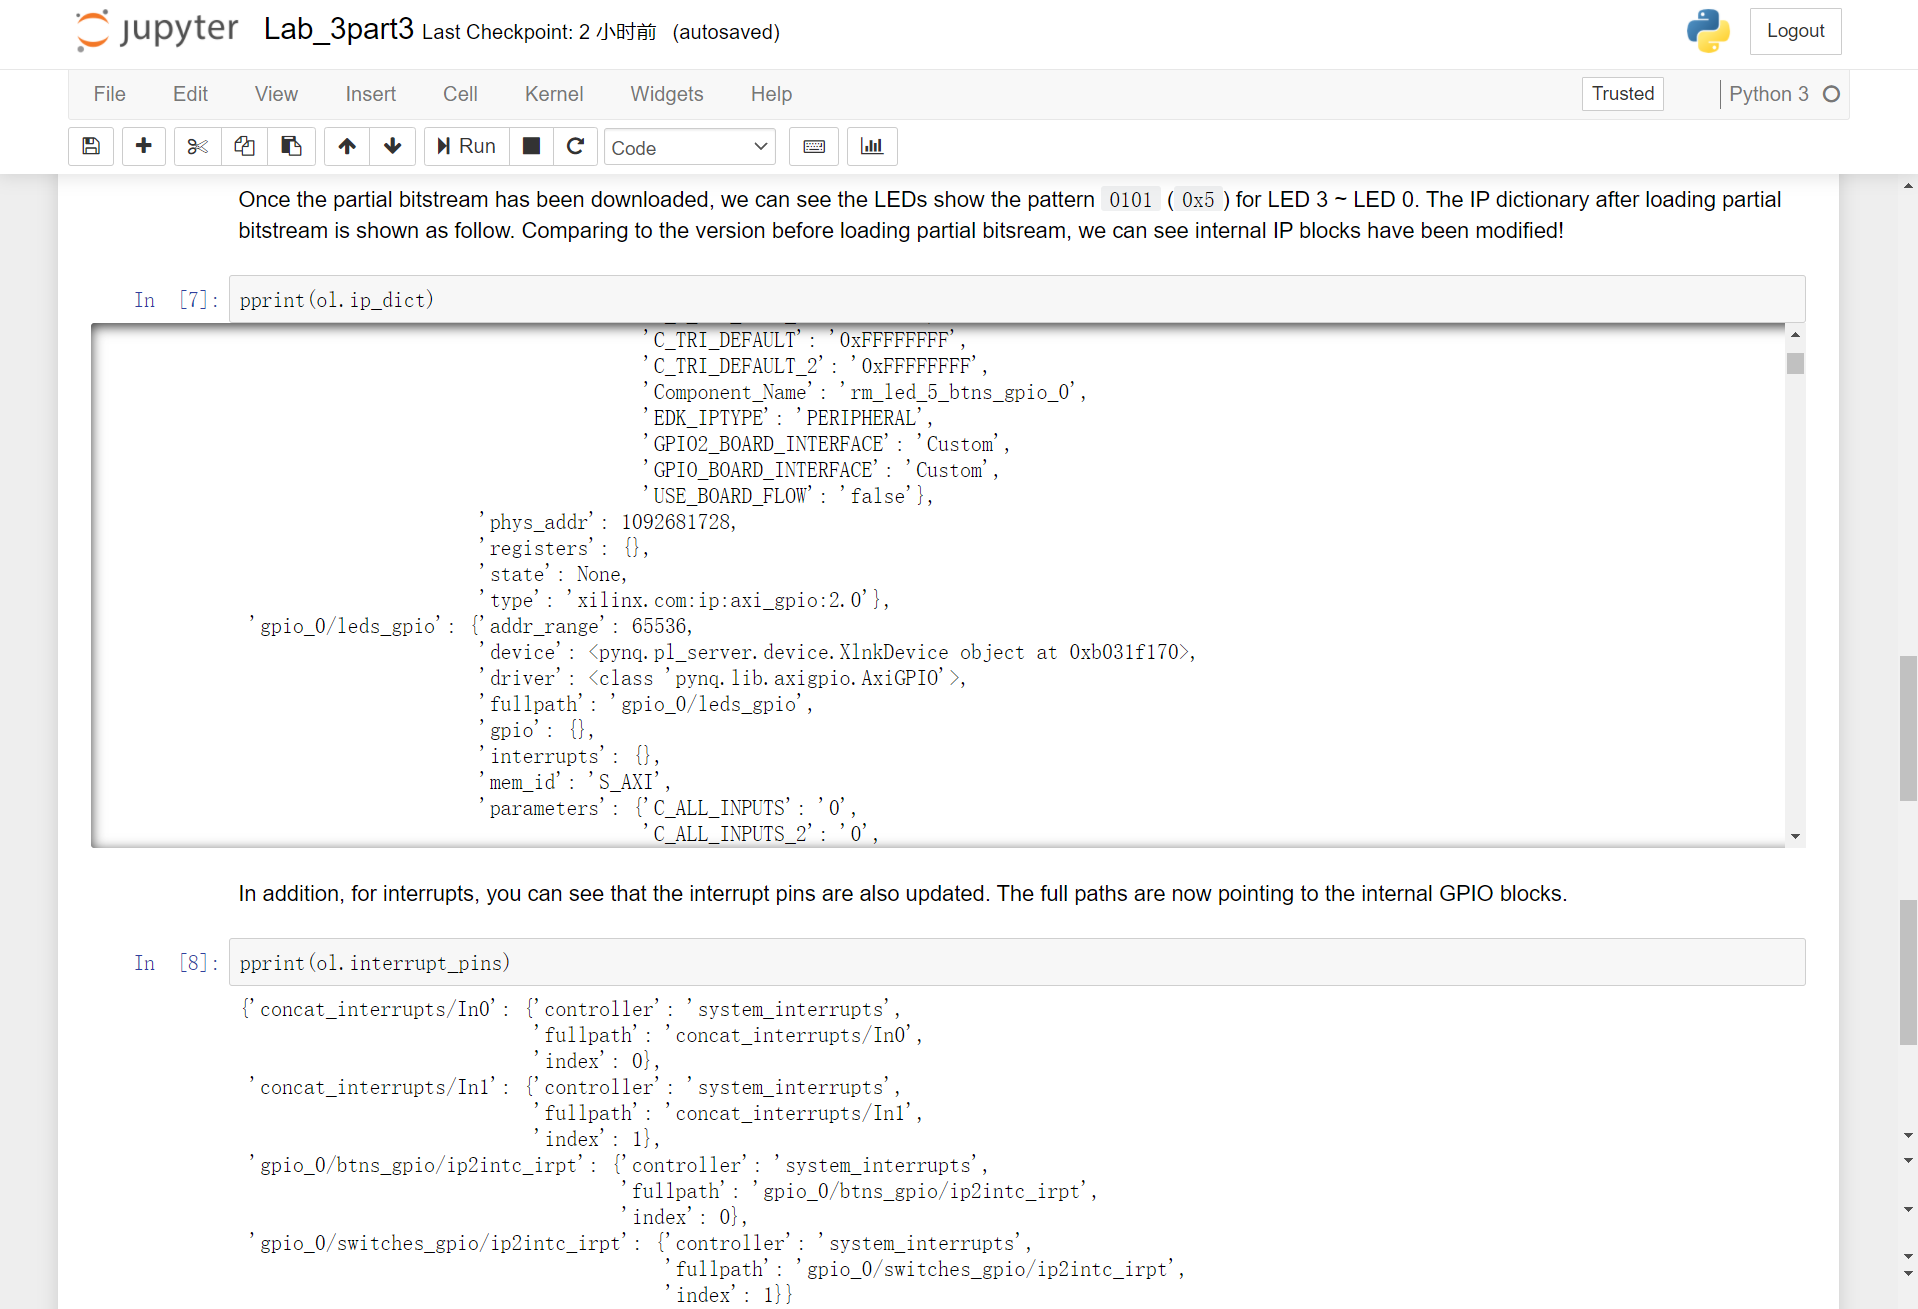
\includegraphics[width=1\textwidth]{2.png}
    \caption{Screenshot that shows partial bit stream is loaded.}
\end{figure}
After loading partial bitstream, we find that both internal IP block hierarchy and interrupt pins have been modified. Besides, after partial reconfiguration, the LEDs on Zynq board shows pattern of 0101:
\begin{figure}[H]
    \centering
    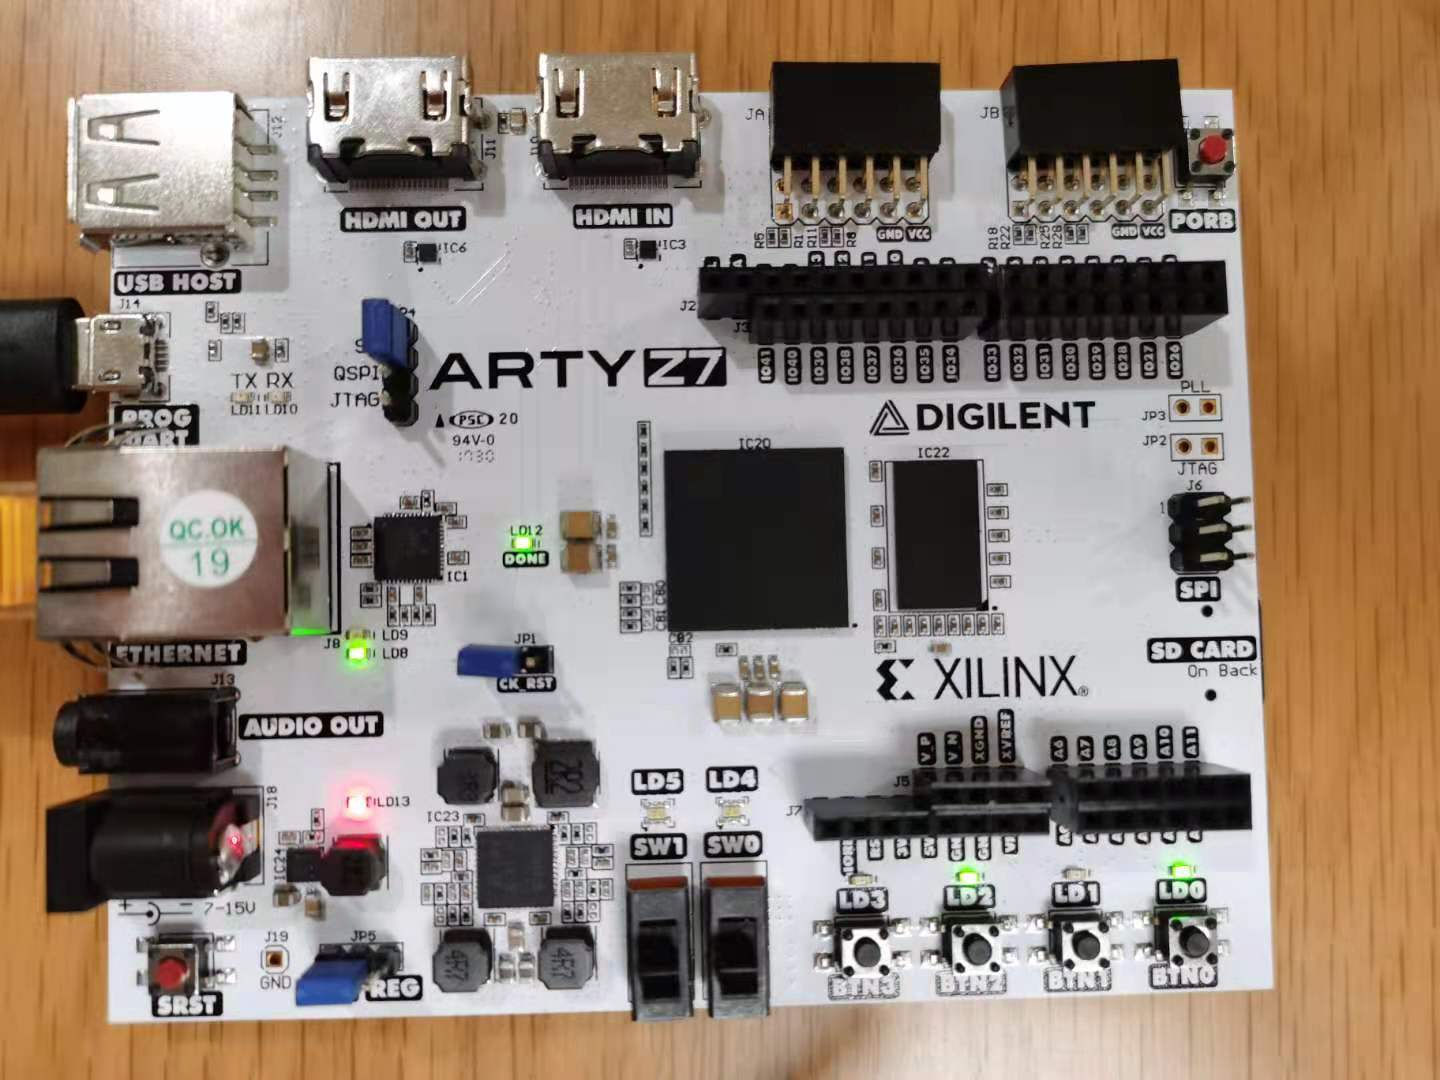
\includegraphics[width=0.8\textwidth]{2-2.jpg}
    \caption{Photo of LED pattern on board after partial reconfiguration}
\end{figure}
\section{PYNQ-Helloworld}
\begin{figure}[H]
    \centering
    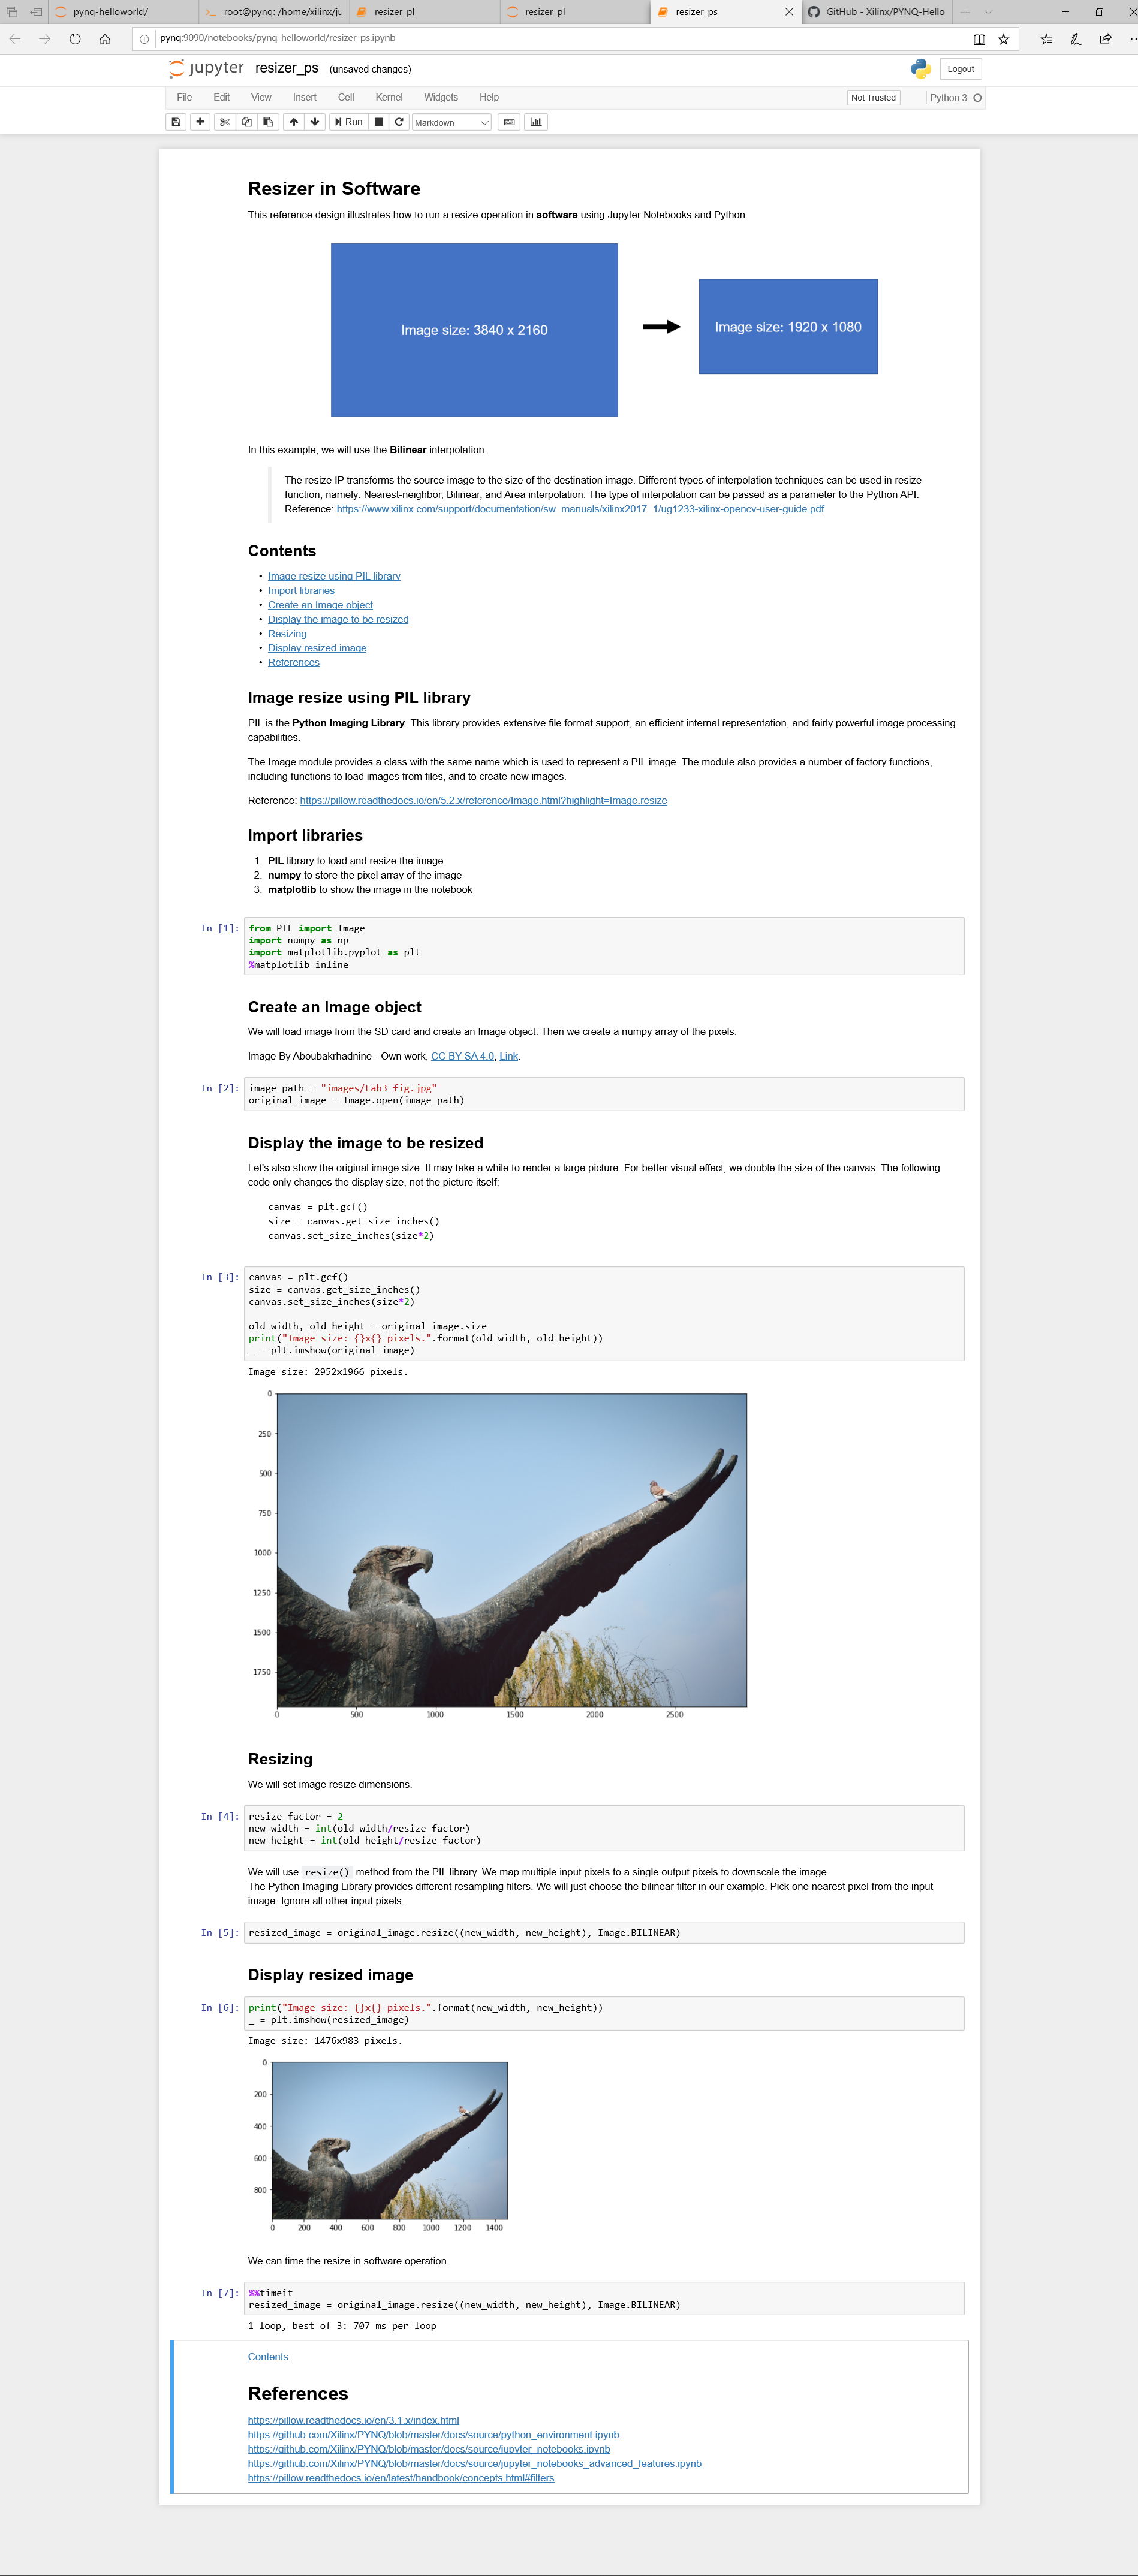
\includegraphics[width=0.7\textwidth]{3.png}
    \caption{A screen shot of the software accelerated resizing.}
\end{figure}
\begin{figure}[H]
    \centering
    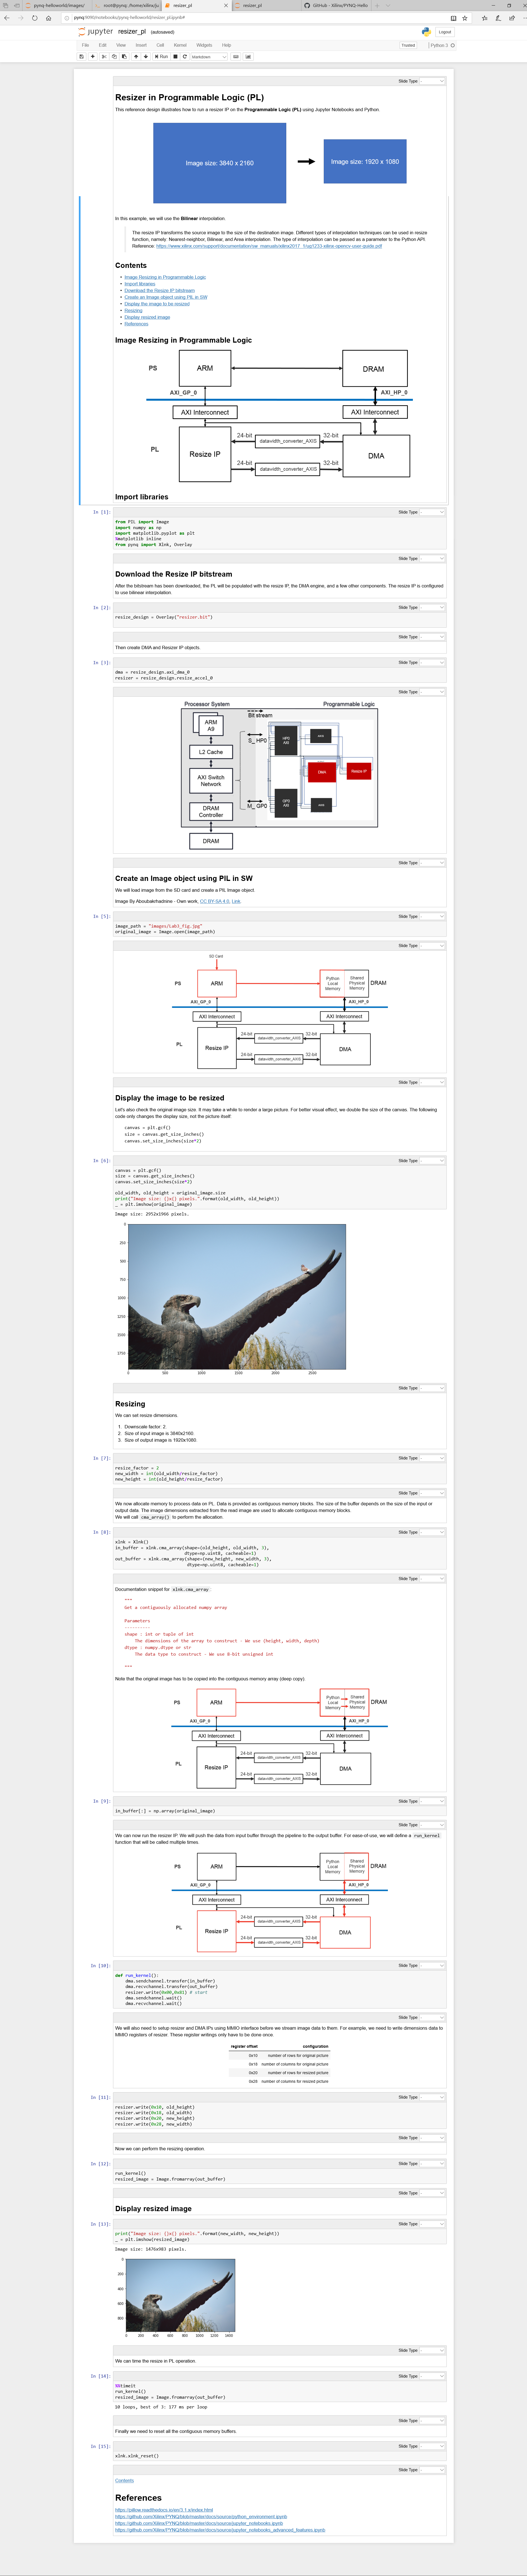
\includegraphics[width=0.33\textwidth]{4.png}
    \caption{A screen shot of the hardware accelerated resizing.}
\end{figure}
As we can see in the figures above, the best loop in software is 3.707 ms while the beat loop in hardware acceleration is 3.177 ms.
\section{Creating Overlays}
The whole overlay package that we created: \url{https://github.com/yihuajack/PYNQ-Adder}. This Github repository includes our code for part 5. 
\begin{figure}[H]
    \centering
    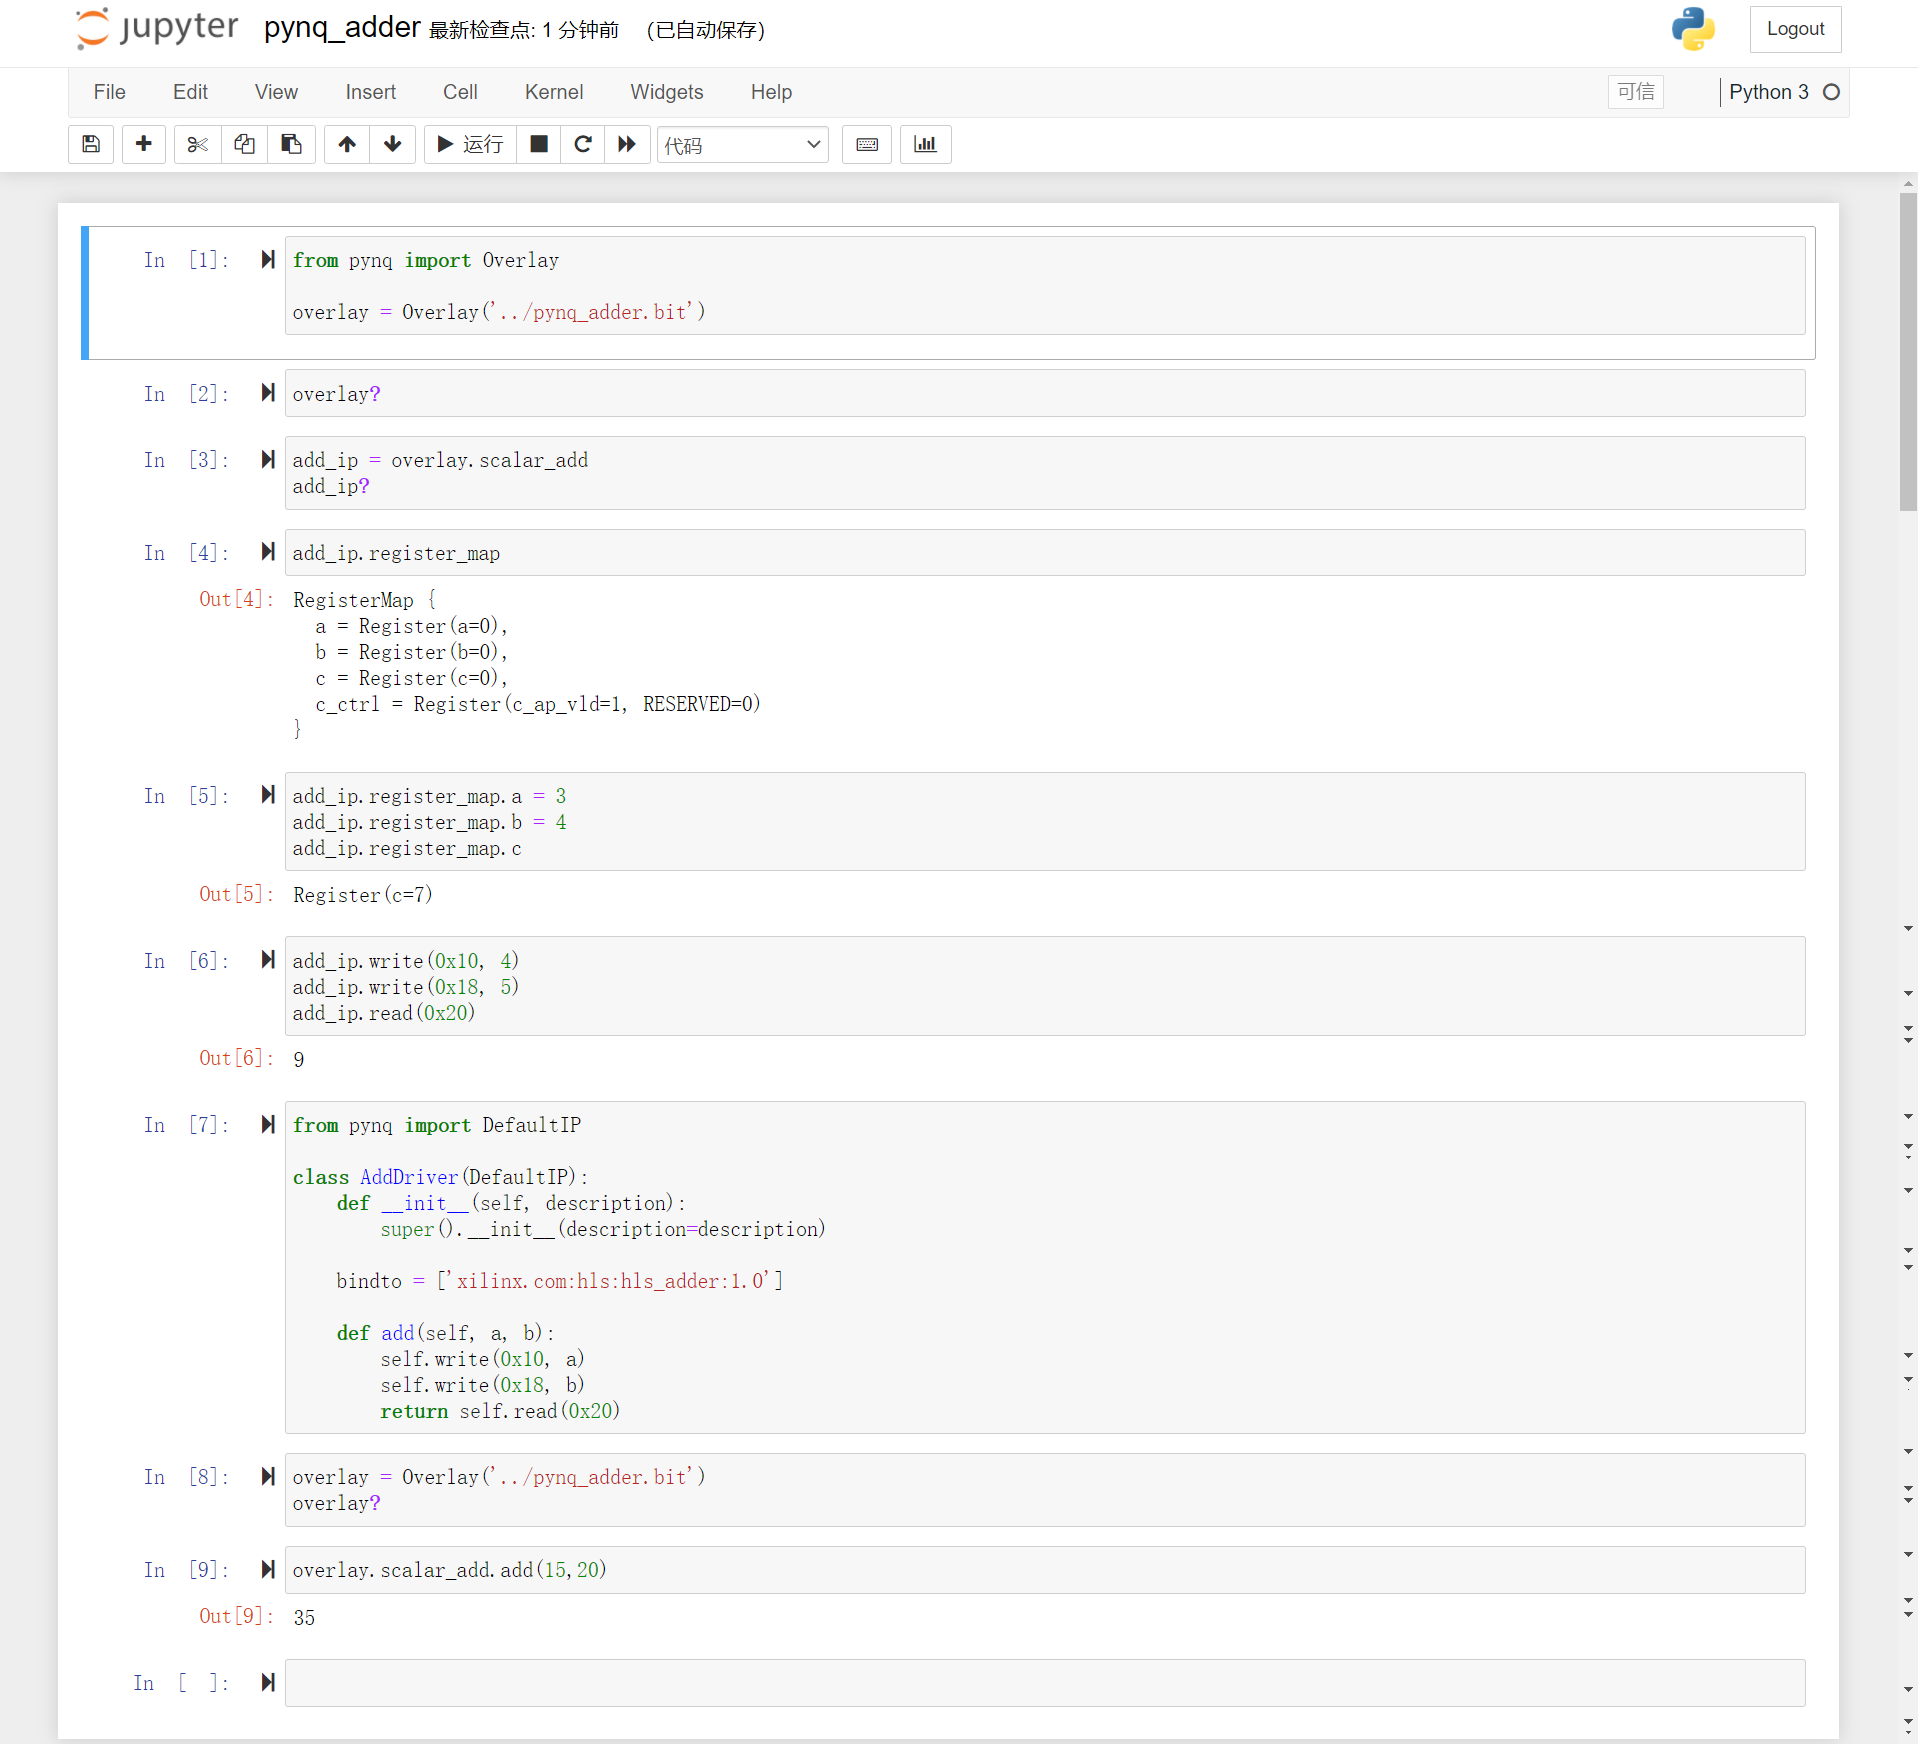
\includegraphics[width=1\textwidth]{5.png}
    \caption{Screenshot that shows your overlay works.}
\end{figure}
\section{Questions}
\begin{enumerate}
\item Please list out any advantages of using overlay.\\
Overlay can be regarded as hardware package. By using it, software engineers can simply use different overlays to handle known problems. It is easy to use without the knowledge of hardware designs.
\item In general, when you choose software approach vs. hardware acceleration approach, what are the considerations? Any tradeoffs?\\
Software is a simpler one by just import the corresponding Python module or other software resources. Hardware acceleration needs a designed ip programmed in the programmable logic and use boards like Arty-7z to finish the task. Hardware acceleration is faster if there is a certain deigned overlay. However, it is not always the case. In contrast, the software acceleration adapts more task requirements and it do not need any external device.
\end{enumerate}
\printbibliography
\end{document}
